\section{Hybrid Filtering Model(CB and CF)}
Hybrid Filtering model is a combination of content-based, collaborative filtering and popular items. 
by any user  The work-flow of the hybrid technique is depicted in the \autoref{fig:hybrid}.
\begin{figure}[H]
	\centering
	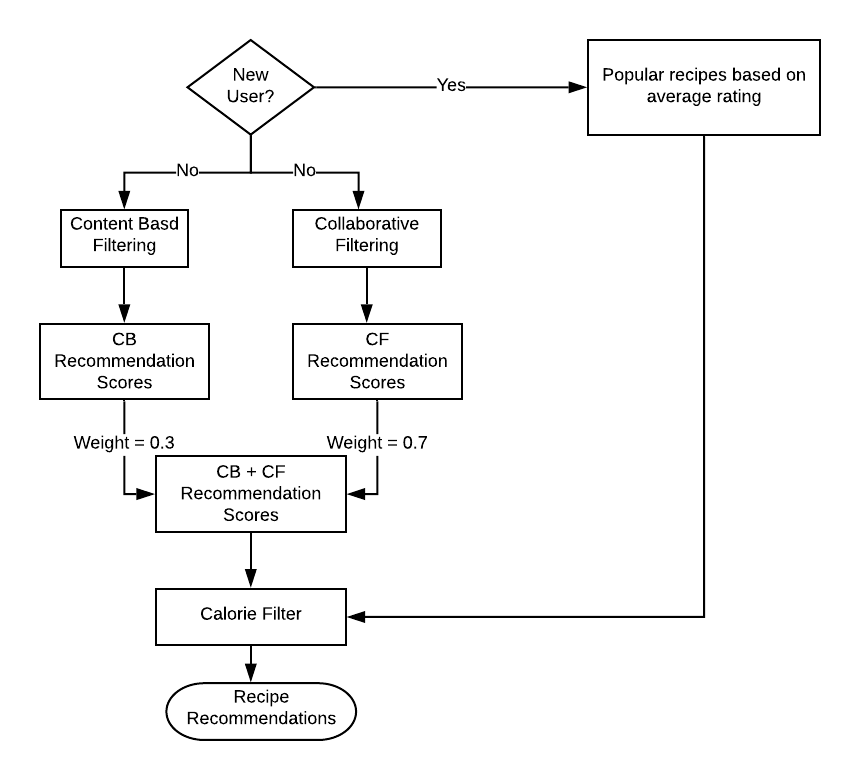
\includegraphics[width=1.0 \linewidth]{hybrid}
	\caption{Hybrid Work-Flow }
	\label{fig:hybrid}
\end{figure}  
\begin{itemize}
\item The system prompts to enter a user id. The existence of an entered user id is cross-verified by the system.
\item If a user id exists, content-based model runs for this user and generates scores for relevant recipes. Once the content-based execution finished, the collaborative filtering model runs and generates predicted ratings for all users. From this result set, predictions for a requested user are filtered out. 
\item Further, scores generated from content-based and predictions generated from collaborative filtering are scaled using 'MinMaxScaler' function of 'sklearn' library.
\item While combining scaled scores, the weighting factor of 0.3 is applied to the content-based and weighting factor 0.7 is applied to the collaborative filtering.
\item The scores are sorted in the descending order to get more relevant items at the top. At this point, recipes that are already rated by the user are omitted. Next, a calorie filter was applied to filter out healthy recipes.
\item Resultant set of recipes is offered as recommendations to the user.
\item If entered user id does not exist in the system, the system prompts to enter user details such as 'height in inches', 'weight in lbs', 'age', 'gender' and lifestyle choice option. User BMR and calorie intake per dish are calculated as discussed in the \nameref{sec:user_info}. 
\item The popularity-based algorithm compares the calorie requirements for user and then filter out recipes based on the user's calorie requirement. The resultant set of recipes represented as recommendations to the user. 
\item System provides an option to give feedback for a recipe in the form of ratings. The user can submit a recipe name with a rating. This feedback generates user profile and recommends recipes based on the combination of content-based and collaborative filtering.
\end{itemize}
